\chapter{Direction Cosines and Direction Angles}

\begin{center}
    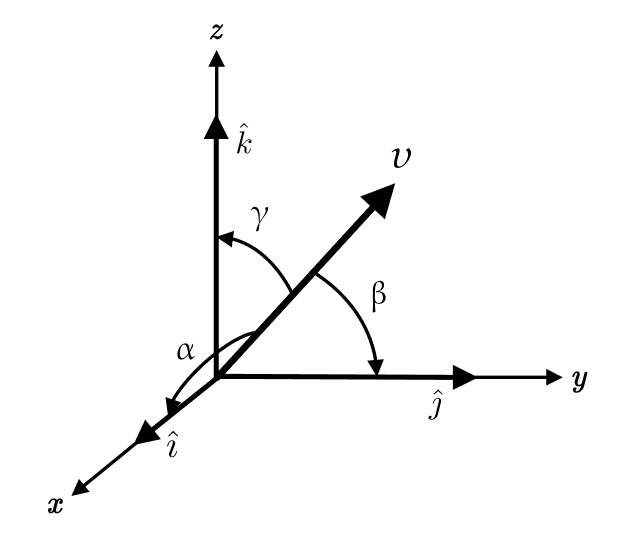
\includegraphics[scale=0.25]{assets/Direction_cosine_vector 1.png}
\end{center}

Direction angles are angles that a vector makes with the unit vectors
$\hat{\imath}$, $\hat{\jmath}$ and $\hat{k}$, denoted by $\alpha$, $\beta$ and
$\gamma$ respectively. In other words, $alpha$, $\beta$ and $\gamma$ are the
angles between the vector and the $x$, $y$ and $z$ axis respectively.

Recall the formula for the dot product of two vectors $\vec{v}$ and $\vec{u}$\[ \vec{v} \cdot \vec{u} = \norm{\vec{v}} \norm{\vec{u}} \cos\theta\] where $\theta$ is the angle between the two vectors.

Let's calculate the dot product of $\vec{v}$ and $\hat{\imath}$.
\begin{align*}
    \vec{v} \cdot \hat{\imath}                                  & = \norm{\vec{v}} \norm{\hat{\imath}} \cos\alpha \\
    \langle v_1, v_2, v_3 \rangle \cdot \langle 1, 0, 0 \rangle & = \norm{\vec{v}} \times 1 \times \cos\alpha     \\
    v_1                                                         & = \norm{\vec{v}} \cos\alpha                     \\
    \cos\alpha                                                  & = \frac{v_1}{\norm{\vec{v}}}
\end{align*}

\newpage
Similarly, we can calculate the dot product of $\vec{v}$ and $\hat{\jmath}$ and
$\hat{k}$ in the same way. Hence, we can conclude that \[\cos\alpha = \frac{v_1}{\norm{\vec{v}}} \qquad \cos\beta = \frac{v_2}{\norm{\vec{v}}} \qquad \cos\gamma = \frac{v_3}{\norm{\vec{v}}}\]
These are called the \textbf{direction cosines} of $\vec{v}$.

We can also express any unit vector $\hat{v}$ in terms of its direction
cosines.
\begin{align*}
    \vec{v}                         & = v_1\hat{\imath} + v_2\hat{\jmath} + v_3\hat{k}                                                                         \\
    \dfrac{\vec{v}}{\norm{\vec{v}}} & = \dfrac{v_1}{\norm{\vec{v}}}\hat{\imath} + \dfrac{v_2}{\norm{\vec{v}}}\hat{\jmath} + \dfrac{v_3}{\norm{\vec{v}}}\hat{k} \\
    \hat{v}                         & = \cos\alpha\hat{\imath} + \cos\beta\hat{\jmath} + \cos\gamma\hat{k}
\end{align*}
If we take the magnitude of $\hat{v}$, we get \[\norm{\hat{v}} = \sqrt{\cos^2\alpha + \cos^2\beta + \cos^2\gamma} = 1\] Squaring both sides, we get \[\cos^2\alpha + \cos^2\beta + \cos^2\gamma = 1\]
~\\
\noindent\textbf{Example 1. } Find the direction cosines and direction angles of the vector $\vec{u} = \hat{\imath} + 8\hat{\jmath} + 4\hat{k}$.
\begin{align*}
    \norm{\vec{u}} & = \sqrt{1^2 + 8^2 + 4^2} \\
                   & = \sqrt{81}              \\
                   & = 9
\end{align*}
\vspace{-5em}
\begin{multicols}{2}
    \begin{align*}
        \cos\alpha & = \frac{v_1}{\norm{\vec{v}}} = \frac{1}{9} \\
        \cos\beta  & = \frac{v_2}{\norm{\vec{v}}} = \frac{8}{9} \\
        \cos\gamma & = \frac{v_3}{\norm{\vec{v}}} = \frac{4}{9}
    \end{align*}

    \begin{align*}
        \alpha & = \cos^{-1}\left(\frac{1}{9}\right) \approx 1.459 \text{ rad} \\
        \beta  & = \cos^{-1}\left(\frac{8}{9}\right) \approx 0.476 \text{ rad} \\
        \gamma & = \cos^{-1}\left(\frac{4}{9}\right) \approx 1.110 \text{ rad}
    \end{align*}
\end{multicols}